\documentclass[tikz,border=0pt]{standalone}
\usepackage{iftex}
\ifLuaTeX
\usepackage{fontspec}
\setsansfont{DejaVu Sans}
\else
\usepackage[T1]{fontenc}
\usepackage[utf8]{inputenc}
\usepackage{lmodern}
\fi
\usepackage{amsmath}
\usetikzlibrary{arrows.meta}
\renewcommand{\familydefault}{\sfdefault}
\definecolor{adbg}{HTML}{101827}
\definecolor{adfg}{HTML}{F1F5F9}
\definecolor{admuted}{HTML}{B5C4D9}
\definecolor{adline}{HTML}{A9BDD8}
\definecolor{adgroup}{HTML}{172236}
\definecolor{adborder}{HTML}{435470}
\definecolor{adinput}{HTML}{93C5FD}
\definecolor{adinputfill}{HTML}{202E44}
\definecolor{adcompute}{HTML}{5EEAD4}
\definecolor{adcomputefill}{HTML}{202E44}
\definecolor{admodel}{HTML}{C4B5FD}
\definecolor{admodelfill}{HTML}{202E44}
\definecolor{admemory}{HTML}{7DD3FC}
\definecolor{admemoryfill}{HTML}{202E44}
\definecolor{adtool}{HTML}{FCD34D}
\definecolor{adtoolfill}{HTML}{202E44}
\definecolor{adcontrol}{HTML}{CBD5E1}
\definecolor{adcontrolfill}{HTML}{202E44}
\definecolor{adoutput}{HTML}{6EE7B7}
\definecolor{adoutputfill}{HTML}{202E44}
\definecolor{adneutral}{HTML}{CBD5E1}
\definecolor{adneutralfill}{HTML}{202E44}
\begin{document}
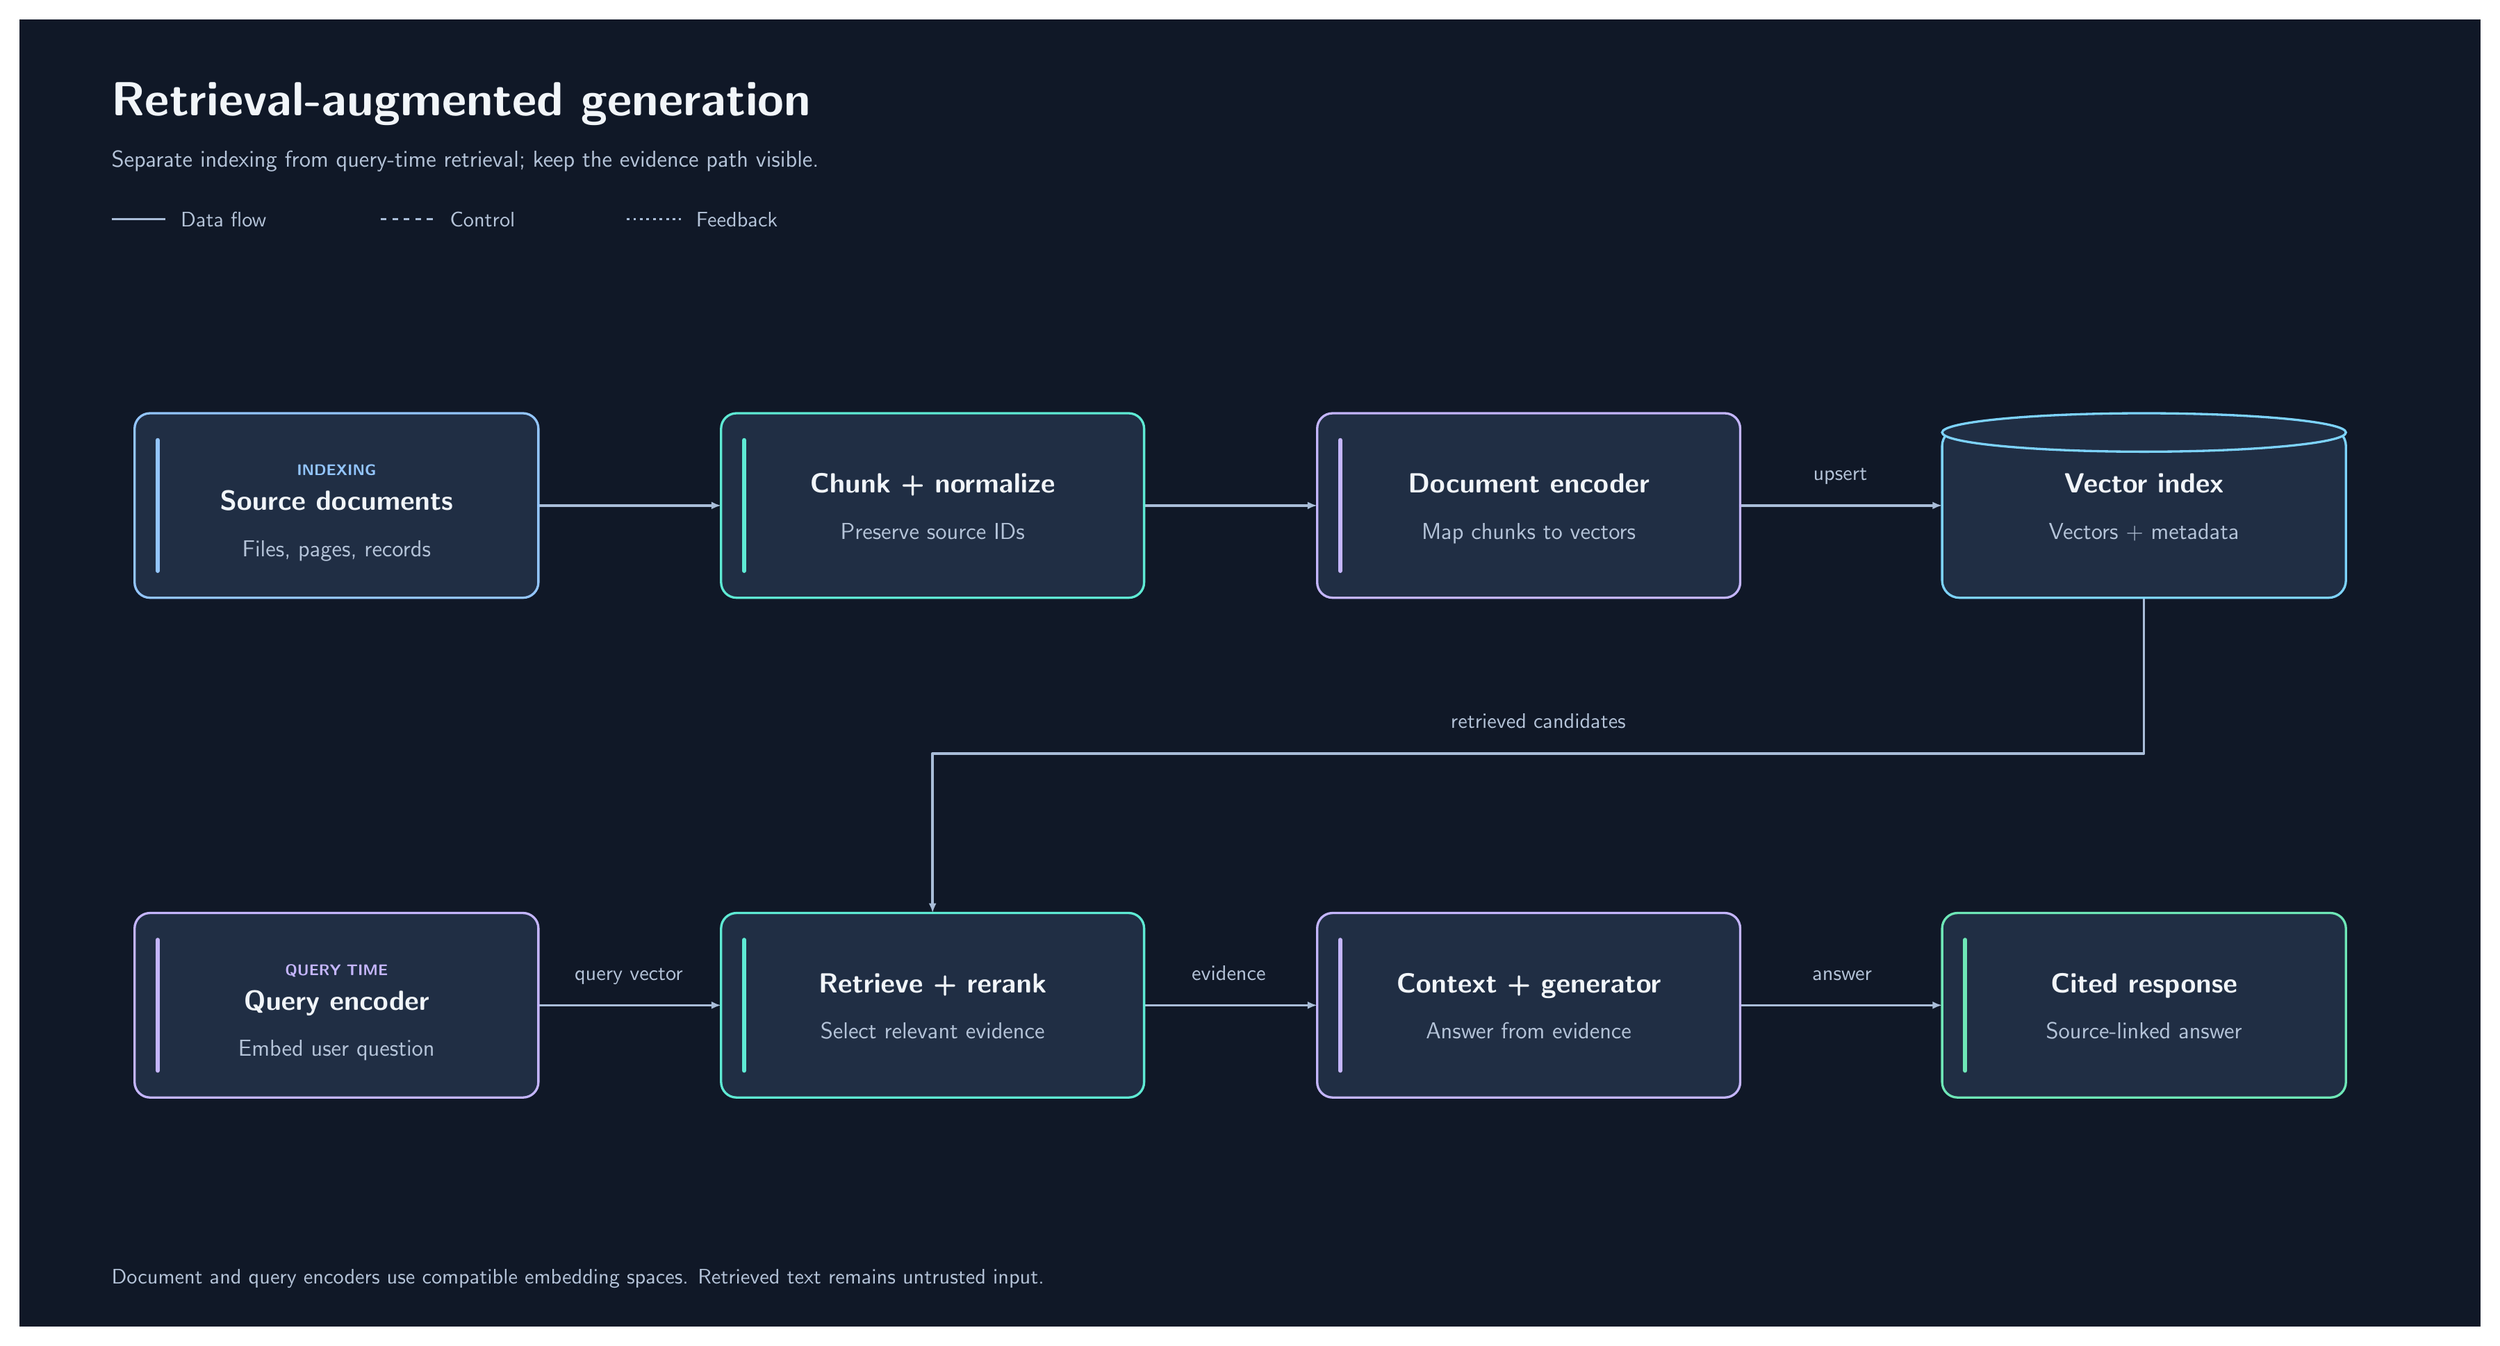
\begin{tikzpicture}[x=1pt,y=-1pt,inner sep=0pt,outer sep=0pt]
\path[use as bounding box] (0,0) rectangle (1280,680);
\fill[adbg] (0,0) rectangle (1280,680);
\node[anchor=base west,text=adfg,font={\sffamily\fontsize{29}{34.8}\selectfont\bfseries}] at (48,50) {Retrieval-augmented generation};
\node[anchor=base west,text=admuted,font={\sffamily\fontsize{13}{15.6}\selectfont}] at (48,77) {Separate indexing from query-time retrieval; keep the evidence path visible.};
\draw[adline,line width=1.4pt] (48,104) -- (76,104);
\node[anchor=base west,text=admuted,font={\sffamily\fontsize{10.5}{12.6}\selectfont}] at (84,108) {Data flow};
\draw[adline,line width=1.4pt,dashed] (188,104) -- (216,104);
\node[anchor=base west,text=admuted,font={\sffamily\fontsize{10.5}{12.6}\selectfont}] at (224,108) {Control};
\draw[adline,line width=1.4pt,dotted] (316,104) -- (344,104);
\node[anchor=base west,text=admuted,font={\sffamily\fontsize{10.5}{12.6}\selectfont}] at (352,108) {Feedback};
\draw[adline,line width=1.3pt,-{Latex[length=5pt,width=4pt]},line join=round] (270,253) -- (317.5,253) -- (365,253);
\draw[adline,line width=1.3pt,-{Latex[length=5pt,width=4pt]},line join=round] (585,253) -- (630,253) -- (675,253);
\draw[adline,line width=1.3pt,-{Latex[length=5pt,width=4pt]},line join=round] (895,253) -- (947.5,253) -- (1000,253);
\draw[adline,line width=1.3pt,-{Latex[length=5pt,width=4pt]},line join=round] (270,513) -- (317.5,513) -- (365,513);
\draw[adline,line width=1.3pt,-{Latex[length=5pt,width=4pt]},line join=round] (1105,301) -- (1105,382) -- (475,382) -- (475,465);
\draw[adline,line width=1.3pt,-{Latex[length=5pt,width=4pt]},line join=round] (585,513) -- (630,513) -- (675,513);
\draw[adline,line width=1.3pt,-{Latex[length=5pt,width=4pt]},line join=round] (895,513) -- (947.5,513) -- (1000,513);
\draw[draw=adinput,fill=adinputfill,line width=1.2pt,rounded corners=8pt] (60,205) rectangle (270,301);
\draw[adinput,line width=2.2pt,line cap=round] (72,219) -- (72,287);
\node[anchor=base,text=adinput,font={\sffamily\fontsize{8.5}{10.2}\selectfont\bfseries}] at (165,237.5) {INDEXING};
\node[anchor=base,text=adfg,font={\sffamily\fontsize{15}{18.0}\selectfont\bfseries}] at (165,255.5) {Source documents};
\node[anchor=base,text=admuted,font={\sffamily\fontsize{11.5}{13.799999999999999}\selectfont}] at (165,279.5) {Files, pages, records};
\draw[draw=adcompute,fill=adcomputefill,line width=1.2pt,rounded corners=8pt] (365,205) rectangle (585,301);
\draw[adcompute,line width=2.2pt,line cap=round] (377,219) -- (377,287);
\node[anchor=base,text=adfg,font={\sffamily\fontsize{15}{18.0}\selectfont\bfseries}] at (475,246.5) {Chunk + normalize};
\node[anchor=base,text=admuted,font={\sffamily\fontsize{11.5}{13.799999999999999}\selectfont}] at (475,270.5) {Preserve source IDs};
\draw[draw=admodel,fill=admodelfill,line width=1.2pt,rounded corners=8pt] (675,205) rectangle (895,301);
\draw[admodel,line width=2.2pt,line cap=round] (687,219) -- (687,287);
\node[anchor=base,text=adfg,font={\sffamily\fontsize{15}{18.0}\selectfont\bfseries}] at (785,246.5) {Document encoder};
\node[anchor=base,text=admuted,font={\sffamily\fontsize{11.5}{13.799999999999999}\selectfont}] at (785,270.5) {Map chunks to vectors};
\draw[draw=admemory,fill=admemoryfill,line width=1.2pt,rounded corners=9pt] (1000,213) rectangle (1210,301);
\draw[draw=admemory,fill=admemoryfill,line width=1.2pt] (1105,215) ellipse [x radius=105pt,y radius=10pt];
\node[anchor=base,text=adfg,font={\sffamily\fontsize{15}{18.0}\selectfont\bfseries}] at (1105,246.5) {Vector index};
\node[anchor=base,text=admuted,font={\sffamily\fontsize{11.5}{13.799999999999999}\selectfont}] at (1105,270.5) {Vectors + metadata};
\draw[draw=admodel,fill=admodelfill,line width=1.2pt,rounded corners=8pt] (60,465) rectangle (270,561);
\draw[admodel,line width=2.2pt,line cap=round] (72,479) -- (72,547);
\node[anchor=base,text=admodel,font={\sffamily\fontsize{8.5}{10.2}\selectfont\bfseries}] at (165,497.5) {QUERY TIME};
\node[anchor=base,text=adfg,font={\sffamily\fontsize{15}{18.0}\selectfont\bfseries}] at (165,515.5) {Query encoder};
\node[anchor=base,text=admuted,font={\sffamily\fontsize{11.5}{13.799999999999999}\selectfont}] at (165,539.5) {Embed user question};
\draw[draw=adcompute,fill=adcomputefill,line width=1.2pt,rounded corners=8pt] (365,465) rectangle (585,561);
\draw[adcompute,line width=2.2pt,line cap=round] (377,479) -- (377,547);
\node[anchor=base,text=adfg,font={\sffamily\fontsize{15}{18.0}\selectfont\bfseries}] at (475,506.5) {Retrieve + rerank};
\node[anchor=base,text=admuted,font={\sffamily\fontsize{11.5}{13.799999999999999}\selectfont}] at (475,530.5) {Select relevant evidence};
\draw[draw=admodel,fill=admodelfill,line width=1.2pt,rounded corners=8pt] (675,465) rectangle (895,561);
\draw[admodel,line width=2.2pt,line cap=round] (687,479) -- (687,547);
\node[anchor=base,text=adfg,font={\sffamily\fontsize{15}{18.0}\selectfont\bfseries}] at (785,506.5) {Context + generator};
\node[anchor=base,text=admuted,font={\sffamily\fontsize{11.5}{13.799999999999999}\selectfont}] at (785,530.5) {Answer from evidence};
\draw[draw=adoutput,fill=adoutputfill,line width=1.2pt,rounded corners=8pt] (1000,465) rectangle (1210,561);
\draw[adoutput,line width=2.2pt,line cap=round] (1012,479) -- (1012,547);
\node[anchor=base,text=adfg,font={\sffamily\fontsize{15}{18.0}\selectfont\bfseries}] at (1105,506.5) {Cited response};
\node[anchor=base,text=admuted,font={\sffamily\fontsize{11.5}{13.799999999999999}\selectfont}] at (1105,530.5) {Source-linked answer};
\fill[adbg,rounded corners=4pt] (920.1,226) rectangle (973.9,246);
\node[anchor=base,text=admuted,font={\sffamily\fontsize{11}{13.2}\selectfont}] at (947,240) {upsert};
\fill[adbg,rounded corners=4pt] (271.2,486) rectangle (362.8,506);
\node[anchor=base,text=admuted,font={\sffamily\fontsize{11}{13.2}\selectfont}] at (317,500) {query vector};
\fill[adbg,rounded corners=4pt] (719,355) rectangle (861,375);
\node[anchor=base,text=admuted,font={\sffamily\fontsize{11}{13.2}\selectfont}] at (790,369) {retrieved candidates};
\fill[adbg,rounded corners=4pt] (595.8,486) rectangle (662.2,506);
\node[anchor=base,text=admuted,font={\sffamily\fontsize{11}{13.2}\selectfont}] at (629,500) {evidence};
\fill[adbg,rounded corners=4pt] (921.1,486) rectangle (974.9,506);
\node[anchor=base,text=admuted,font={\sffamily\fontsize{11}{13.2}\selectfont}] at (948,500) {answer};
\node[anchor=base west,text=admuted,font={\sffamily\fontsize{11}{13.2}\selectfont}] at (48,658) {Document and query encoders use compatible embedding spaces. Retrieved text remains untrusted input.};
\end{tikzpicture}
\end{document}
